%%%%%%%%%%%%%%%%%%%%%%%%%%%%%%%%%%%%%%%%%
% Arsclassica Article
% LaTeX Template
% Version 1.1 (1/8/17)
%
% This template has been downloaded from:
% http://www.LaTeXTemplates.com
%
% Original author:
% Lorenzo Pantieri (http://www.lorenzopantieri.net) with extensive modifications by:
% Vel (vel@latextemplates.com)
%
% License:
% CC BY-NC-SA 3.0 (http://creativecommons.org/licenses/by-nc-sa/3.0/)
%
%%%%%%%%%%%%%%%%%%%%%%%%%%%%%%%%%%%%%%%%%

%----------------------------------------------------------------------------------------
%	PACKAGES AND OTHER DOCUMENT CONFIGURATIONS
%----------------------------------------------------------------------------------------

\documentclass[
10pt, % Main document font size
a4paper, % Paper type, use 'letterpaper' for US Letter paper
oneside, % One page layout (no page indentation)
%twoside, % Two page layout (page indentation for binding and different headers)
headinclude,footinclude, % Extra spacing for the header and footer
BCOR5mm, % Binding correction
]{scrartcl}

%%%%%%%%%%%%%%%%%%%%%%%%%%%%%%%%%%%%%%%%%
% Arsclassica Article
% Structure Specification File
%
% This file has been downloaded from:
% http://www.LaTeXTemplates.com
%
% Original author:
% Lorenzo Pantieri (http://www.lorenzopantieri.net) with extensive modifications by:
% Vel (vel@latextemplates.com)
%
% License:
% CC BY-NC-SA 3.0 (http://creativecommons.org/licenses/by-nc-sa/3.0/)
%
%%%%%%%%%%%%%%%%%%%%%%%%%%%%%%%%%%%%%%%%%

%----------------------------------------------------------------------------------------
%	REQUIRED PACKAGES
%----------------------------------------------------------------------------------------

\usepackage[
nochapters, % Turn off chapters since this is an article        
beramono, % Use the Bera Mono font for monospaced text (\texttt)
eulermath,% Use the Euler font for mathematics
pdfspacing, % Makes use of pdftex’ letter spacing capabilities via the microtype package
dottedtoc % Dotted lines leading to the page numbers in the table of contents
]{classicthesis} % The layout is based on the Classic Thesis style

\usepackage{arsclassica} % Modifies the Classic Thesis package

\usepackage[T1]{fontenc} % Use 8-bit encoding that has 256 glyphs

\usepackage[utf8]{inputenc} % Required for including letters with accents

\usepackage{graphicx} % Required for including images
\graphicspath{{Figures/}} % Set the default folder for images

\usepackage{enumitem} % Required for manipulating the whitespace between and within lists

\usepackage{lipsum} % Used for inserting dummy 'Lorem ipsum' text into the template

\usepackage{subfig} % Required for creating figures with multiple parts (subfigures)

\usepackage{amsmath,amssymb,amsthm} % For including math equations, theorems, symbols, etc

\usepackage{varioref} % More descriptive referencing

%----------------------------------------------------------------------------------------
%	\frac{d_t(w_1, N_t^1(u) \backslash N_t^1(v)}{|N_t^1(u)| + d_t(w_1, N_t^2(u))} \times \frac{1}{d_t(w_1)} STYLES
%---------------------------------------------------------------------------------------

\theoremstyle{definition} % Define theorem styles here based on the definition style (used for definitions and examples)
\newtheorem{definition}{Definition}

\theoremstyle{plain} % Define theorem styles here based on the plain style (used for theorems, lemmas, propositions)
\newtheorem{theorem}{Theorem}

\theoremstyle{remark} % Define theorem styles here based on the remark style (used for remarks and notes)

%----------------------------------------------------------------------------------------
%	HYPERLINKS
%---------------------------------------------------------------------------------------

\hypersetup{
%draft, % Uncomment to remove all links (useful for printing in black and white)
colorlinks=true, breaklinks=true, bookmarks=true,bookmarksnumbered,
urlcolor=webbrown, linkcolor=RoyalBlue, citecolor=webgreen, % Link colors
pdftitle={}, % PDF title
pdfauthor={\textcopyright}, % PDF Author
pdfsubject={}, % PDF Subject
pdfkeywords={}, % PDF Keywords
pdfcreator={pdfLaTeX}, % PDF Creator
pdfproducer={LaTeX with hyperref and ClassicThesis} % PDF producer
} % Include the structure.tex file which specified the document structure and layout

\hyphenation{Fortran hy-phen-ation} % Specify custom hyphenation points in words with dashes where you would like hyphenation to occur, or alternatively, don't put any dashes in a word to stop hyphenation altogether

%----------------------------------------------------------------------------------------
%	TITLE AND AUTHOR(S)
%----------------------------------------------------------------------------------------

\title{\normalfont\spacedallcaps{Discovery Through Gossip}} % The article title

%\subtitle{Subtitle} % Uncomment to display a subtitle

\author{\spacedlowsmallcaps{Mohammad Mahzoun}} % The article author(s) - author affiliations need to be specified in the AUTHOR AFFILIATIONS block

\date{\today} % An optional date to appear under the author(s)
\newtheorem{corollary}{Corollary}[theorem]
\newtheorem{lemma}[theorem]{\textbf{Lemma}}
%----------------------------------------------------------------------------------------

\begin{document}

%----------------------------------------------------------------------------------------
%	HEADERS
%----------------------------------------------------------------------------------------

\renewcommand{\sectionmark}[1]{\markright{\spacedlowsmallcaps{#1}}} % The header for all pages (oneside) or for even pages (twoside)
%\renewcommand{\subsectionmark}[1]{\markright{\thesubsection~#1}} % Uncomment when using the twoside option - this modifies the header on odd pages
\lehead{\mbox{\llap{\small\thepage\kern1em\color{halfgray} \vline}\color{halfgray}\hspace{0.5em}\rightmark\hfil}} % The header style

\pagestyle{scrheadings} % Enable the headers specified in this block

%----------------------------------------------------------------------------------------
%	TABLE OF CONTENTS & LISTS OF FIGURES AND TABLES
%----------------------------------------------------------------------------------------

\maketitle % Print the title/author/date block

\setcounter{tocdepth}{2} % Set the depth of the table of contents to show sections and subsections only

\tableofcontents % Print the table of contents

\listoffigures % Print the list of figures

\listoftables % Print the list of tables

%----------------------------------------------------------------------------------------

\newpage % Start the article content on the second page, remove this if you have a longer abstract that goes onto the second page

%----------------------------------------------------------------------------------------
%	INTRODUCTION
%----------------------------------------------------------------------------------------

\section{Introduction}
We want to study Gossip based discovery processes in both directed and undirected graphs using push discovery (triangulation) and pull discovery (two-hop walk process).

\begin{figure}[tb]
	\centering
	\subfloat[Triangulation]{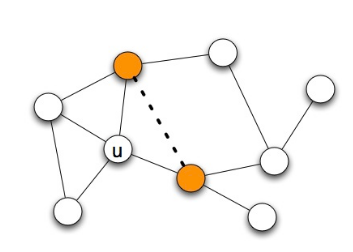
\includegraphics[width=.45\columnwidth]{push}} \quad
	\subfloat[Two-hop walk]{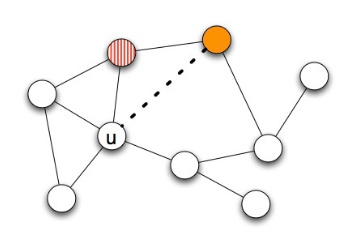
\includegraphics[width=.45\columnwidth]{pull}\label{fig:ipsum}}
	\caption[Discovery Methods]{Discovery Methods} % The text in the square bracket is the caption for the list of figures while the text in the curly brackets is the figure caption
	\label{fig:esempio}
\end{figure}
We are interested in studying the time taken by process to converge to the transitive closure of the graph.
\subsection{Notation}

\begin{table}[hbt]
	\caption{Table of Notations}
	\centering
	\begin{tabular}{llr}
		\cmidrule(r){1-2}
		Notation & Description \\
		\midrule
		$\delta_t$ & Minimum degree of $G_t$  \\
		$N_t^i(u)$ & Set of nodes at distance $i$ from $u$ in $G_t$ \\
		$d_t(u)$ & Degree of $u$ in $G_t$ \\
		$d_t(u, S)$ & Degree induced on $S$ \\
		\bottomrule
	\end{tabular}
	\label{tab:label}
\end{table}

\subsection{Useful lemmas}

\begin{lemma}\label{lem:1}
	$|\cup_{i=1}^{4} N_t^i(u)| \geq min \{ 2\delta_t, n-1\}$ for all $u \in G_t$.
\end{lemma}
\begin{proof}
	If $N_t^3 \ne \emptyset$, then $|\cup_{i=2}^{4} N_t^i(u)| \geq \delta_t$ and $|N_t^1(u)| \geq \delta_t$. So $|\cup_{i=1}^{4} N_t^i(u)| \geq 2\delta_t$ since the two sets are disjoint. \\
	If $N_t^3 = \emptyset$, $N_t^1(u) \cup N_t^2(u) = n-1$ since $G_t$ is connected.
\end{proof}

\begin{lemma}\label{lem:2}
	Consider $k$ Bernoulli experiments in which the success probability of the $ith$ experiment is at least $i/m$ where $m \geq k$. If $X_i$ denotes the number of trials needed for experiment $i$ to output a success and $X = \sum_{i=1}^{k}X_i$, then $Pr[X > (c+1)m\ln m] < \frac{1}{m^c}$.
\end{lemma}
\begin{proof}
	w.l.o.g assume that $k=m$. The problem can be seen as \textit{coupon collector problem} where $X_{m+i-1}$ is the number of steps to collect $ith$ coupon. Consider the probability of not obtaining the $ith$ coupon after $(c+1)m\ln m$ steps, we have:
	\begin{math}
		(1 - \frac{1}{m})^{(c+1) m \ln m} < e^{-(c+1)\ln m} = \frac{1}{m^{c+1}}
	\end{math}
	By union bound, the probability that some coupon has not been collected after $(c+1)m \ln m$ steps is less than $\frac{1}{m^c}$.
\end{proof}

%----------------------------------------------------------------------------------------
%	METHODS
%----------------------------------------------------------------------------------------

\section{Triangulation Results}
\subsection{Upper Bound}

\begin{theorem}[Upper bound for triangulation process]\label{thm:3}
	For any connected undirected graph, the triangulation process converges to a complete graph in $O(n \log^2 n)$ rounds with high probability.
\end{theorem}
In order to prove Theorem \ref{thm:3}, we prove that the minimum degree of the graph increases by a constant factor (or equals to $n-1$) in $O(n\log n)$ steps. We say that a node $v$ is \textbf{weakly tied} to a set of nodes $S$ if $d_t(v, S) < \delta_0 / 2$, and \textbf{strongly tied} to a set of nodes $S$ if $d_t(v, S) \geq \delta_0 / 2$.

\begin{lemma}\label{lem:4}
	If $d_t(u) < \min \{n-1, (1+\frac{1}{4} \delta_0)\} $ and $w \in N_t^1(u)$ has at least $\frac{\delta_0}{4}$ edges to $N_t^2(u)$, then the probability that $u$ connects to a node in $N_t^2(u)$ through $w$ in round $t$ is at least $\frac{1}{6n}$.
\end{lemma}
\begin{proof}
	The probability that $u$ connects to a node in $N_t^2(u)$ through $w$ in round $t$ is: \\
	\begin{center}
	\begin{math}
		\frac{d_t(w, N_t^2(u))}{D_t(w)} \times \frac{1}{d_t(w)} \geq
		\frac{d_t(w, N_t^2(u))}{D_t(w)} \times \frac{1}{n} \geq
		\frac{d_t(w, N_t^2(u))}{|N_t^1(u)|+ d_t(w, N_t^2(u))} \times \frac{1}{n} \geq
		\frac{d_t(w, N_t^2(u))}{(1 + \frac{1}{4})\delta_0 + d_t(w, N_t^2(u))} \times \frac{1}{n} \geq
		\frac{ \frac{\delta_0}{4} }{(1 + \frac{1}{4})\delta_0 + \frac{\delta_0}{4}} \times \frac{1}{n} =
			\frac{1}{6n}
	\end{math}
	\end{center}
\end{proof}

\begin{lemma}\label{lem:5}
	If $d_t(u) < \min \{n-1, (1+\frac{1}{4} \delta_0)\} $ and $w \in N_t^1(u)$ is weakly tied to $N_t^2(u)$, and $v \in N_0^2(u) \cap N_0^1(w)$, then $u$ connects to $v$ through $w$ in round $t$ with probability at least $\frac{1}{4\delta_0^2}$.
\end{lemma}
\begin{proof}
	Since $w$ is weakly tied to $N_t^2(u)$ and $d_t(w)$ is at most $|N_t^1(u)|+ d_t(w, N_t^2(u))$, we obtain that $d_t(w)$ is at most $(1 + \frac{1}{4})\delta_0 + \frac{\delta_0}{2}$. Therefore, the probability that $u$ connects to $v$ through $w$ in round $t$ equals:
	\begin{center}
		\begin{math}
			\frac{1}{d_t(w)^2} \geq
			\frac{1}{((1 + \frac{1}{4})\delta_0 + \frac{\delta_0}{2})^2} \geq
			\frac{1}{\frac{7\delta_0}{4}^2} \geq
			\frac{1}{4\delta_0^2}.
		\end{math}
	\end{center}
\end{proof}
To analyze the growth in the degree of a node $u$, we consider two overlapping cases. The first case is when more than $\delta_0/4$ nodes of $N_t^1(u)$ are strongly tied to $N_t^2(u)$, and the second is when less than $\delta_0/3$ nodes of $N_t^1(u)$ are strongly tied to $N_t^2(u)$. 


\begin{lemma}[Several nodes are strongly tied to two-hop neighbors]\label{lem:6}
	There exists a $T = O(n \log n)$ such that if more than $\frac{\delta_0}{4}$ nodes in $N_t^1(u)$ each have at least $\frac{\delta_0}{4}$ edges to $N_t^2(u)$ for all $t < T$, then with probability at least $1 - \frac{1}{n^2}$ it holds that $d_T(u) \geq \min \{n-1, (1+\frac{1}{4})\delta_0 \}$.
\end{lemma}
\begin{proof}
	We assume that $d_t(u) < \min \{n-1, (1+\frac{1}{4})\delta_0 \}$ for all $ t < T$. (Otherwise there is nothing to prove). Let $w \in N_t^1 (u)$ be a node that has at least $\frac{\delta_0}{4}$ edges to $N_t^2(u)$. By Lemma \ref{lem:4} we know that: 
	\begin{center}
		Pr[$u$ connects to a node in $N_t^2(u)$ through $w$ in round $t$] $ \geq \frac{1}{6n}$
	\end{center} 
There are more than $\frac{\delta_0}{4}$ such $w$'s in $N_t^1(u)$, each of which independently executes a triangulation step in any given round. Consider $T = \frac{72n\ln n}{\delta_0}$. We have $18n\ln n$ chances to add an edge between $u$ and a node in $N_t^2(u)$. Thus, 
\begin{center}
	Pr[$u$ connects to a node in $N_t^2(u)$ after $T$ rounds] $\geq
	1 - (1 - \frac{1}{6n})^{18n\ln n}$ \\ $\geq 
	1 - e^{-3\ln n} = 1 - \frac{1}{n^3}$.
\end{center} 
If a node that is two hops away from $u$ becomes a neighbor of $u$ by round $t$, it is no longer in $N_t^2(u)$. Therefore, in $T = T_1\frac{\delta_0}{4} = O(n\log n)$ rounds, $u$ will connect to at least $\frac{\delta_0}{4}$ new nodes with probability at least $1 - \frac{1}{n^2}$ and $d_T(u) \geq (1+\frac{1}{4})\delta_0$
\end{proof}

\begin{lemma}[Few neighbors are strongly tied to two-hop neighbors]\label{lem:7}
	There exists $T = O(n\log n)$ such that if less than $\frac{\delta_0}{3}$ nodes in $N_t^1(u)$ are strongly tied to $N_t^2(u)$ for all $t < T$, and there exists a node $v_0 \in N_0^1(u)$ that is strongly tied to $N_0^2(u)$, then $d_T(u) \geq \min \{n-1, (1+\frac{1}{8})\delta_0 \}$ with probability at least $ 1 - \frac{1}{n^2}$.
\end{lemma}
\begin{proof}
	Let $T, T_1, T_2 = O(n\log n)$. We assume $d_t(u) < \min \{n-1, (1+\frac{1}{8})\delta_0 \}$ for all $t < T$. Let $S_t^0$ denote the set of $v_0$'s neighbors in $N_t^2(u)$ which are strongly tied to $N_t^1(u)$ at round $t$ and $W_t^0$ denote the set of $v_0$'s neighbors in $N_t^2(u)$ which are weakly tied to $N_t^1(u)$ at round $t$.\\
	Consider $v \in S_t^0$. Less than $\frac{\delta_0}{3}$ nodes in $N_t^1(u)$ are strongly tied to $N_t^2(u)$ (hype), thus more than $\frac{\delta_0}{2} - \frac{\delta_0}{3} = \frac{\delta_0}{6}$ neighbors of $v$ in $N_t^1(u)$ are weakly tied to $N_t^2(u)$. Let $w$ be such node. By Lemma \ref{lem:5}, the probability that $u$ connects to $v$ through $w$ in round $t$ is at least $\frac{1}{4\delta_0^2}$. We have at least $\frac{\delta_0}{6}$ choices for $w$, each of which executes a triangulation step each round. Consider $T_1 = 72\delta_0\ln n$ rounds of the process. Then the probability that u connects to $v$  in $T_1$ rounds is at least:
	\begin{center}
		\begin{math}
		1 - (1 - \frac{1}{4\delta_0^2}) ^{12\delta_0^2\ln n} \geq
		1 - e^{-3\ln n} = 1 - \frac{1}{n^3}.
		\end{math}
	\end{center}
	Thus if there exists $t < T_2$ such that $|S_t^0| \geq \frac{\delta_0}{8}$, then in $T_1 + T_2$ rounds, $d_{T_1 + T_2}(u) \geq (1 + \frac{1}{8}) \delta_0$ with probability at least $1 - \frac{1}{n^2}$. This implies the claim of the lemma if we set $T = T_1 + T_2$.\\
	Therefore, let $S_t^0 < \frac{\delta_0}{8}$ for all $t \leq T_2$. Define $R_t^0 = R_{t-1}^0 \cup W_t^0, R_0^0 = W_0^0$. If at least $\frac{\delta_0}{8}$ nodes in $R_t^0$ are connected to $u$ at any time $t \leq T_2$, then the claim of the lemma holds. Consider $|R_t^0 \cap N_t^1(u)| < \delta_0 / 8$ for all $ t \leq T_2$. Consider any round $t \leq T_2$. From the definition of $R_t^0$, we have:
	\begin{center}
		\begin{math}
		|R_t^0| \geq |W_t^0| = d_t(v_0, N_t^2(u)) - |S_t^0| \geq d_t(v_0, N_t^2(u)) - \frac{\delta_0}{8}. 
		\end{math}
	\end{center}
	At round $0$, $v_0$ is strongly tied to $N_0^2(u)$, i.e., $d_0(v_0, N_0^2(u)) \geq \frac{\delta_0}{2}$.
	Since $\delta_0 \leq d_t(u) < (1 + 1/8)\delta_0$, we have:
	\begin{center}
		\begin{math}
		d_t(v_0, N_t^2(u)) \geq d_t(v_0, N_0^2(u)) - \delta_0 / 8 \geq 3\delta_0/8.
		\end{math}
	\end{center}	
	let $e_1$ denote the event [$u$ connect to a node in $R_t^0 \backslash N_t^1(u)$ through $v_0$ in round t].
	\begin{center}
	 	\begin{math}
	 		Pr[e_1] = \frac{|R_t^0 \backslash N_t^1(u)|}{d_t(v_0)} \times \frac{1}{d_t(v_0)} = 
	 		\frac{|R_t^0| - |R_t^0 \cap C_t^1(u)|}{d_t(v_0)} \times \frac{1}{d_t(v_0)} \geq
	 		\frac{|R_t^0| - |R_t^0 \cap C_t^1(u)|}{d_t(v_0)|} \times \frac{1}{n} \geq
	 		\frac{|R_t^0| - |R_t^0 \cap C_t^1(u)|}{|N_t^1(u)| + d_t(v_0, N_t^2(u))} \times \frac{1}{n} \geq
	 		\frac{|R_t^0| - \delta_0/8}{|N_t^1(u)| + d_t(v_0, N_t^2(u))} \times \frac{1}{n} \geq
	 		\frac{d_t(v_0, N_t^2(u)) - \delta_0/8 - \delta_0/8}{|N_t^1(u)| + d_t(v_0, N_t^2(u))} \times \frac{1}{n} \geq 
	 		\frac{3\delta_0/8 - \delta_0/8}{|N_t^1(u)| + 3\delta_0/8} \times \frac{1}{n} \geq
	 		\frac{3\delta_0/8 - \delta_0/8}{(1+ 1/8)\delta_0 + 3\delta_0/8} \times \frac{1}{n} = 
	 		\frac{1}{12n}.
	 	\end{math}
	\end{center}
	Let $X_1$ be the number of rounds it takes for $e_1$ to occur and let $v_1$ denote a witness for $e_1$. Since $v_1$ is in $R_{X_1}^0$, it is also in $W_{t_1}^0$ for some $t_1 \leq X_1$. Therefore, $v_1$ is weakly tied to $N_{t_1}^1(u)$ and strongly tied to $N_{t_1}^2(u) \cup N_{t_1}^3(u)$ at the start of round $t_1$. Thus, at the start of round $t_1$, $v_1$ has at least $\delta_0/2$ neighbors that are not neighbors of $u$. 
	If $d_t(v_1, N_t^2(u)) < 3\delta_0/8$ for any round t $X_1 \leq t \leq T_2$, then at least $\delta_0/2 - 3\delta_0/8 = \delta_0/8$ neighbors of $v_1$ that were not neighbors of $u$ at the start of round $t_1$ became neighbors of $u$ by the start of round $t$. This would imply that $d_t(u) \geq (1 + 1/8)\delta_0$ which violates the assumption at the start of the proof. So consider the case where $d_t(v_1, N_t^2(u)) \geq 3\delta_0/8$ for all $X_1 \leq t \leq T_2$. Let $S_t^1(W_t^1)$ denote the set of $v_1$'s neighbors in $N_t^2(u)$ that are strongly(weakly) tied to $N_t^1(u)$. If $|S_t^1| \geq \delta_0 / 8$ for any $t \leq T_2$, then as for the case $|S_t^0| \geq \delta_0 / 8$, in at most $T_1 + T_2$ rounds, the degree of $u$ is at least $(1+ 1/8)\delta_0$ with probability at least $1 - \frac{1}{n^2}$.\\
	So assume that $|S_t^1| < \delta_0 / 8$ for all $t \leq T_2$. Consider a round $t$ such that $X_1 \leq t \leq T_2$. 
	Define $R_t^1 = R_{t-1}^1 \cup W_t^1, R_{t_1}^1 = W_{t_1}^1$. Let $e_2$ denote the event [$u$ connect to a node in $R_t^0 \backslash N_t^1(u)$ or $R_t^1 \backslash N_t^1(u)$through $v_0$ or $v_1$ in round t]. By the same calculation as for $v_0$, we have $Pr[e_2] \geq 2/12n$, as long as $T_2 \geq X_1 + X_2$. Similarly, we define $e_3, \ldots, e_{\lceil \delta_0/8 \rceil}$ and $X_3, \ldots, X_{\lceil \delta_0/8 \rceil}$, and obtain that  $Pr[i_2] \geq i/12n$ for $ 1 \leq i \leq \lceil \delta_0/8 \rceil$, as long as $T_2 \geq \sum_{j = 1}^{i}X_j$. The total number of rounds for $u$ to gain at least $\delta_0/8$ nodes as neighbors is given by $\sum_{i = 1}^{\lceil \delta_0/8 \rceil}X_i$, which, according to Lemma \ref{lem:2}, is bounded by $36n\ln n$ with probability at least $1 - \frac{1}{n^2}$. So setting $T_2 = 36n\ln n$ and $T = T_1 + T_2$ completes the proof.	
\end{proof}

\begin{lemma}[All neighbors are weakly tied to two-hop neighbors]\label{lem:8}
	There exists a $T = O(n\log n)$ such that if all nodes in $N_t^1(u)$ are weakly tied to $N_t^2(u)$ for all $t < T$, then with probability at least $1 - \frac{1}{n^2}$ it holds that $d_T(u) \geq \min \{(1+ 1/8)\delta_0, n - 1\}$.
\end{lemma}
\begin{proof}
	Assume $d_t(u) < \min \{(1+ 1/8)\delta_0, n - 1\}$ for all $t < T$. We first show that any node $v \in N_0^2(u)$ will have at least $\delta_0/4$ edges to $N_{T_1}^1(u)$, where $T_1 = O(n\log n)$. After that, $v$ will connect to $u$ in $T_2 = O(n\log n)$ rounds. Therefore, the total number of rounds for $v$ to connect to $u$ is $T_3 = T_1 + T_2 = O(n\log n)$. \\
	Node $v$ at least connects to one node in $N_0^1(u)$. Call it $w_1$. Because all nodes in $N_t^1(u)$ are weakly tied to $N_t^2(u)$, we ave $d_t(w_1, N_t^1(u)) \geq \delta_0 - \delta_0/2 = \delta_0 /2 $. If $d_t(w_1, N_t^1(u)) \backslash N_t^1(v) < \delta_0/4$, then $v$ already has $\delta_0/4$ edges to $N_t^1(u)$. So consider the case where $d_t(w_1, N_t^1(u) \backslash N_t^1(v)) \geq \delta_0/4$. Consider the event $e_1=$ [$v$ connects to a node in $N_t^1(u) \backslash N_t^1(v)$ through $w_1$] and obtain for its probability:
	\begin{center}
		\begin{math}
			Pr[e_1] = \frac{d_t(w_1, N_t^1(u) \backslash N_t^1(v)}{d_t(w_1)} \times \frac{1}{d_t(w_1)} \geq
			\frac{d_t(w_1, N_t^1(u) \backslash N_t^1(v)}{|N_t^1(u)| + d_t(w_1, N_t^2(u))} \times \frac{1}{d_t(w_1)} \geq 
			\frac{\delta_0/4}{(1+1/8)\delta_0 + \delta_0/2} \times \frac{1}{d_t(w_1)} \geq
			\frac{2}{13} \times \frac{1}{n} > \frac{1}{7n}.
		\end{math}
	\end{center}
	Let $X_1$ be the number of rounds needed for $e_1$ to happen and $w_2$ be the witness for it. By our choice, $w_2$ is also weakly tied to $N_t^2(u)$. With the same argument as above, we have $d_t(w_2,  N_t^1(u) \backslash N_t^1(v)) \geq \delta_0/4$. Let $e_2$ denote the event  [$v$ connects to a node in $N_t^1(u)$ through $w_1$ or $w_2$]. We have $Pr[e_2] \geq 2/7n$. Let $X_2$ be the number of rounds needed for $e_2$ to occur. Similarly, define $e_3, X_3, \ldots, e_{\delta_0/4}, X_{\delta_0/4}$ and show that $Pr[e_i] \geq i/7n$. Let $T_1 = \sum_{i}X_i$, which is the bound on the number of rounds needed for $v$ to have at least $\delta_0/4$ neighbors in $N_t^1(u)$. By Lemma \ref{lem:5}, the probability that $u$ connects to $v$ through $w_i$ in round $t$ is at least $\frac{1}{4\delta_0^2}$. There are $\delta_0/4$ such $w_i$'s independently running a triangulation step each round. Consider $T_2 = 48\delta_0 \ln n$ rounds of the process, Then:
	\begin{center}
		Pr[$u$ connects to $v$ in $T_2$ rounds] $\geq 1 - (1 - \frac{1}{4\delta_0^2})^{12\delta_0^2 \ln n} \geq 1- \frac{1}{n^3}$.
	\end{center}
	So each $v \in N_0^2(u)$ will connect to $u$ in round $T_3 = T_1 + T_2$ with probability at least $1 - \frac{1}{n^3}$. So in round $T_3$, $u$ will connect to all nodes in $N_0^2(u)$ with probability at least $1 - \frac{|N_0^2(u)}{n^3}$. Then, $N_0^2(u) \subseteq N_{T_3}^1(u), N_0^3(u) \subseteq N_{T_3}^1(u) \cup N_{T_3}^2(u), N_0^4(u) \subseteq N_{T_3}^1(u) \cup N_{T_3}^2(u) \cup  N_{T_3}^3(u)$. We apply the above analysis twice, and obtain that in round $T = 3T_3 = O(n\log n), N_0^2(u) \cup N_0^3(u) \cup  N_0^4(u) \subseteq N_T^1(u)$ with probability at least $ 1 - \frac{1}{n^2}$. By Lemma \ref{lem:1}, $| N_0^2(u) \cup N_0^3(u) \cup  N_0^4(u)| \geq \min\{2\delta_0, n-1\}$.
\end{proof}

Now we can prove Theorem \ref{thm:3}.
\begin{proof}[Proof of Theorem \ref{thm:3}]
	We show that in $O(n\log n)$ rounds, either the graph becomes complete or its minimum degree increases by a factor of at least $1/8$. Then we apply this argument $O(\log n)$ times to complete the proof.\\
	For each $u$ where $d_0(u) < \min \{(1+1/8)\delta_0, n - 1\}$, we consider two cases. Let $S$ be the set of nodes in $N_0^1(u)$ that are strongly tied to $N_0^2(u)$. The first case is when $|S| > \delta_0/3$. By Lemma \ref{lem:6}, there exists $T = O(n \log n)$ such that if at least $\delta_0/4$ nodes in $N_t^1(u)$ have each at least $\delta_0/4$ edges to $N_t^2(u)$ for all $t < T$, then $d_T(u) \geq (1+1/8)\delta_0$ with probability at least $ 1 - \frac{1}{n^2}$. So if every node is $S$ has at least $\delta_0/4$ edges to $N_t^2(u)$ for all $ t < T$, the desired claim of lemma holds. On the other hand, if there is a node in $S$ that has fewer than $\delta_0/4$ edges to $N_t^2(u)$ for some $t < T$, then $u$ has gained at least $\delta_0/2 - \delta_0/4 = \delta_0/4$ new neighbors, giving the desired claim. \\
	If $S < \delta_0/3$, we have two cases. If we remain in this case for $T = O(n \log n)$ rounds and fine a node $v_0 \in N_0^1(u)$ that is strongly tied to $N_T^2(u)$, then by Lemma \ref{lem:7}, we have $d_T(u) \geq \min \{(1+1/8)\delta_0, n - 1\}$ with probability at least $1 - \frac{1}{n^2}$. Otherwise, by Lemma \ref{lem:8}, $T = O(n \log n)$ exists such that if we remain in this case for $T$ rounds, then $d_T(u) \geq  \min \{(1+1/8)\delta_0, n - 1\}$ with probability at least $1 - \frac{1}{n^2}$. Using the union bound, we obtain $\delta_T \geq \min \{(1+1/8)\delta_0, n - 1\}$ in $T = O(n \log n)$ rounds with probability at least $1 - 1/n$. Apply the above argument $O(\log n)$ times to obtain the desired upper bound.
\end{proof}

\subsection{Lower Bound}
\begin{theorem}[Lower bound for triangulation process]\label{thm:9}
	For any connected undirected graph $G$ that has $k \geq 1$ edges less than the complete graph, the triangulation process takes $\Omega(n\log k)$ steps to complete with probability at least $1 - O(e^{-k^{1/4}})$.
\end{theorem}
\begin{proof}
	During the triangulation process, there is a time $t$ when the number of missing edges is at least $m = \Omega(\sqrt{k})$ and the minimum degree is at least $n/3$. If $K < 2n/3$, then this is true initially and for larger $k$, this is true at the first time $t$ the minimum degree is large enough. The second case follows since the degree of a node can at most double in each step guaranteeing that the minimum degree is not larger than $2n/3$ at time $t$ also implying that at least $n/3 = \Omega(k)$ edges are still missing.\\
	Given the bound on the minimum degree, any missing edge $\{u,v\}$ is added by a fixed node $w$ with probability at most $\frac{18}{n^2}$. Since there are $n-2$ such nodes, the probability that a missing edges get added is at most $18/n$. Let $X_i$ be the random variable counting the number of steps needed until the $ith$ of  $m$ missing edges is added. We would like to analyze $Pr[X_1 \leq T, \ldots, X_m \leq T]$ for an appropriate $T$. We have $Pr[X_1 \leq T] \leq 1 - (1 - 18/n)^T \leq 1 - \frac{1}{\sqrt{m}}$ for $ T = \Omega(n\log m)$. Thus:
	\begin{center}
		\begin{math}
		Pr[X_1 \leq T, \ldots, X_m \leq T] = Pr[X_1 \leq T | X_2 \leq T, \ldots, X_m \leq T]\times \ldots \times Pr[X_m \leq T] \leq (1 - \frac{1}{\sqrt{m}})^ m = O(e^{-\sqrt{m}}) = O(e^{-k^{1/4}}).
		\end{math}
	\end{center}
	This shows that the triangulation process takes with probability at least $1 - O(e^{-k^{1/4}})$ at least $\Omega(n \log m) = \Omega(n \log k)$ steps to complete.
\end{proof}

\section{The Two-Hop Walk Results}
\subsection{Upper Bound}
\begin{lemma}[When two-hop neighborhood is not too large]\label{lem:10}
	If $N_t^2(u) < \delta_0/3$, there exists $T = O(n\log n)$ such that with probability at least $1 - 1/n^2$, we have $|N_T^2(u)| \geq \delta_0/3$ or $d_T(u) \geq \min \{2\delta_0, n-1\}$.
\end{lemma}
\begin{proof}
	Omitted.
\end{proof}
\begin{lemma}[When two-hop neighborhood is not too small]\label{lem:11}
	If $N_t^2(u) \geq \delta_0/4$, there exists $T = O(n\log n)$ such that with probability at least $1 - 1/n^2$, we have $|N_T^2(u)| < \delta_0/4$ or $d_T(u) \geq \min \{(1+1/8)\delta_0, n-1\}$.
\end{lemma}
\begin{proof}
	Omitted.
\end{proof}

\begin{theorem}[Upper bound for two-hop walk process]\label{thm:12}
	For connected undirected graphs, the two-hop walk process completes in $O(n\log^2 n)$ rounds with high probability. 
\end{theorem}
\begin{proof}
	In time $T = O(n\log n)$, the minimum degree of the graph increases by a factor of $1/8$. For each $u$ that $d_0(u) < \min \{(1+1/8)\delta_0, n-1\}$, we analyze by the two following cases. First, if $N_0^2(u) \geq \delta_0/2$, by Lemma \ref{lem:11} we know as long as $|N_t^2(u)| \geq \delta_0/4$ for all $t \geq 0$, $d_T(u) \geq \min \{(1+1/8)\delta_0, n-1\}$ with probability $1 - 1/n^2$ where $T = O(n \log n)$. If the condition is not satisfied, we know at least $\delta_0/4$ nodes in $N_0^2(u)$ have been moved to $N_T^1(u)$, which means that $d_T(u) \geq \min \{(1+1/8)\delta_0, n-1\}.$ \\
	Second, If $N_0^2(u) < \delta_0/2$,  by Lemma \ref{lem:10} we know as long as $|N_t^2(u)| < \delta_0/2$ for all $t \geq 0$,  $d_T(u) \geq \min \{(1+1/8)\delta_0, n-1\}$ with probability $1 - 1/n^2$ where $T = O(n \log n)$. 
	If the condition is not satisfied, we are back to analysis in the first case. So with probability $ 1 - 1/n$ the minimum degree of $G$ will become at least $\min \{(1+1/8)\delta_0, n-1\}$. Now we apply the argument $O(\log n)$ times to show that the two-hop process completes in $O(n\log^2n)$ steps with high probability. 
\end{proof}

\subsection{Lower Bound}
\begin{theorem}[Lower bound for two-hop walk process]\label{thm:13}
	For any connected undirected graph $G$ that has $k \geq 1$ edges less than the complete graph, the two-hop process takes $\Omega(n\log k)$ steps to complete with probability at least $1 - O(e^{-k^{1/4}})$.
\end{theorem}
\begin{proof}
	Omitted. Same as the proof of Theorem \ref{thm:9}. 
\end{proof}

%----------------------------------------------------------------------------------------
%	BIBLIOGRAPHY
%----------------------------------------------------------------------------------------

\renewcommand{\refname}{\spacedlowsmallcaps{References}} % For modifying the bibliography heading

\bibliographystyle{unsrt}

\bibliography{sample.bib} % The file containing the bibliography

%----------------------------------------------------------------------------------------

\end{document}